\chapter{Design}
\label{chapter:design}

This chapter presents an in-depth discussion of the system's design, examining the overall architecture, the rationale behind key design decisions, and the unique aspects that distinguish this project. The design of the system is inherently modular, partitioning functionality into clearly defined subsystems that interact through well-specified interfaces. This approach not only promotes ease of development and testing but also facilitates future expansion and maintenance.

\section{System Architecture Overview}

At a high level, the system comprises several loosely coupled components that work together to recreate a local multiplayer experience in a remote gaming context. The primary subsystems include:

\begin{itemize}
	\item \textbf{Controller Input Relay}
	      A custom Python script acts as an intermediary, capturing input events (such as accelerometer data, IR signals, and button presses) using the \texttt{xwiimote} library\cite{xwiimote} and translating them into a binary format. These updates are transmitted over UDP to a wiimote emulator that runs on the host Raspberry Pi.

	\item \textbf{Wiimote Emulator:}
	      The emulator, derived from a fork\cite{jr_wiimote_emu} of the \texttt{WiimoteEmulator} project\cite{wiimote_emulator}, has been extended to handle IR and accelerometer data, bridging the gap between physical inputs and the emulated control signals expected by the Wii. The emulator processes incoming UDP packets, updates its internal state, and generates the corresponding output signals.

	\item \textbf{Audio and Video Streaming:}
	      To recreate the authentic gaming experience, the system includes an audiovisual streaming component. Using the Real-time Transport Protocol (RTP), the video and audio outputs from the host are captured and transmitted to a client device. A significant design challenge was the trade-off between stream quality and latency, leading to a careful tuning of encoding parameters and RTP settings.

	\item \textbf{Automation and Deployment:}
	      An automation script ensures that all system configurations—such as loading kernel modules and setting up environment variables—are applied consistently across devices. This not only simplifies the initial setup but also mitigates issues that might arise from manual configuration errors.
\end{itemize}

\section{Component-Level Design and Data Flow}

The system’s architecture emphasises clear data flow and modularity. Figure~\ref{fig:architecture} illustrates the primary components and their interactions.

\begin{figure}[h]
	\centering
	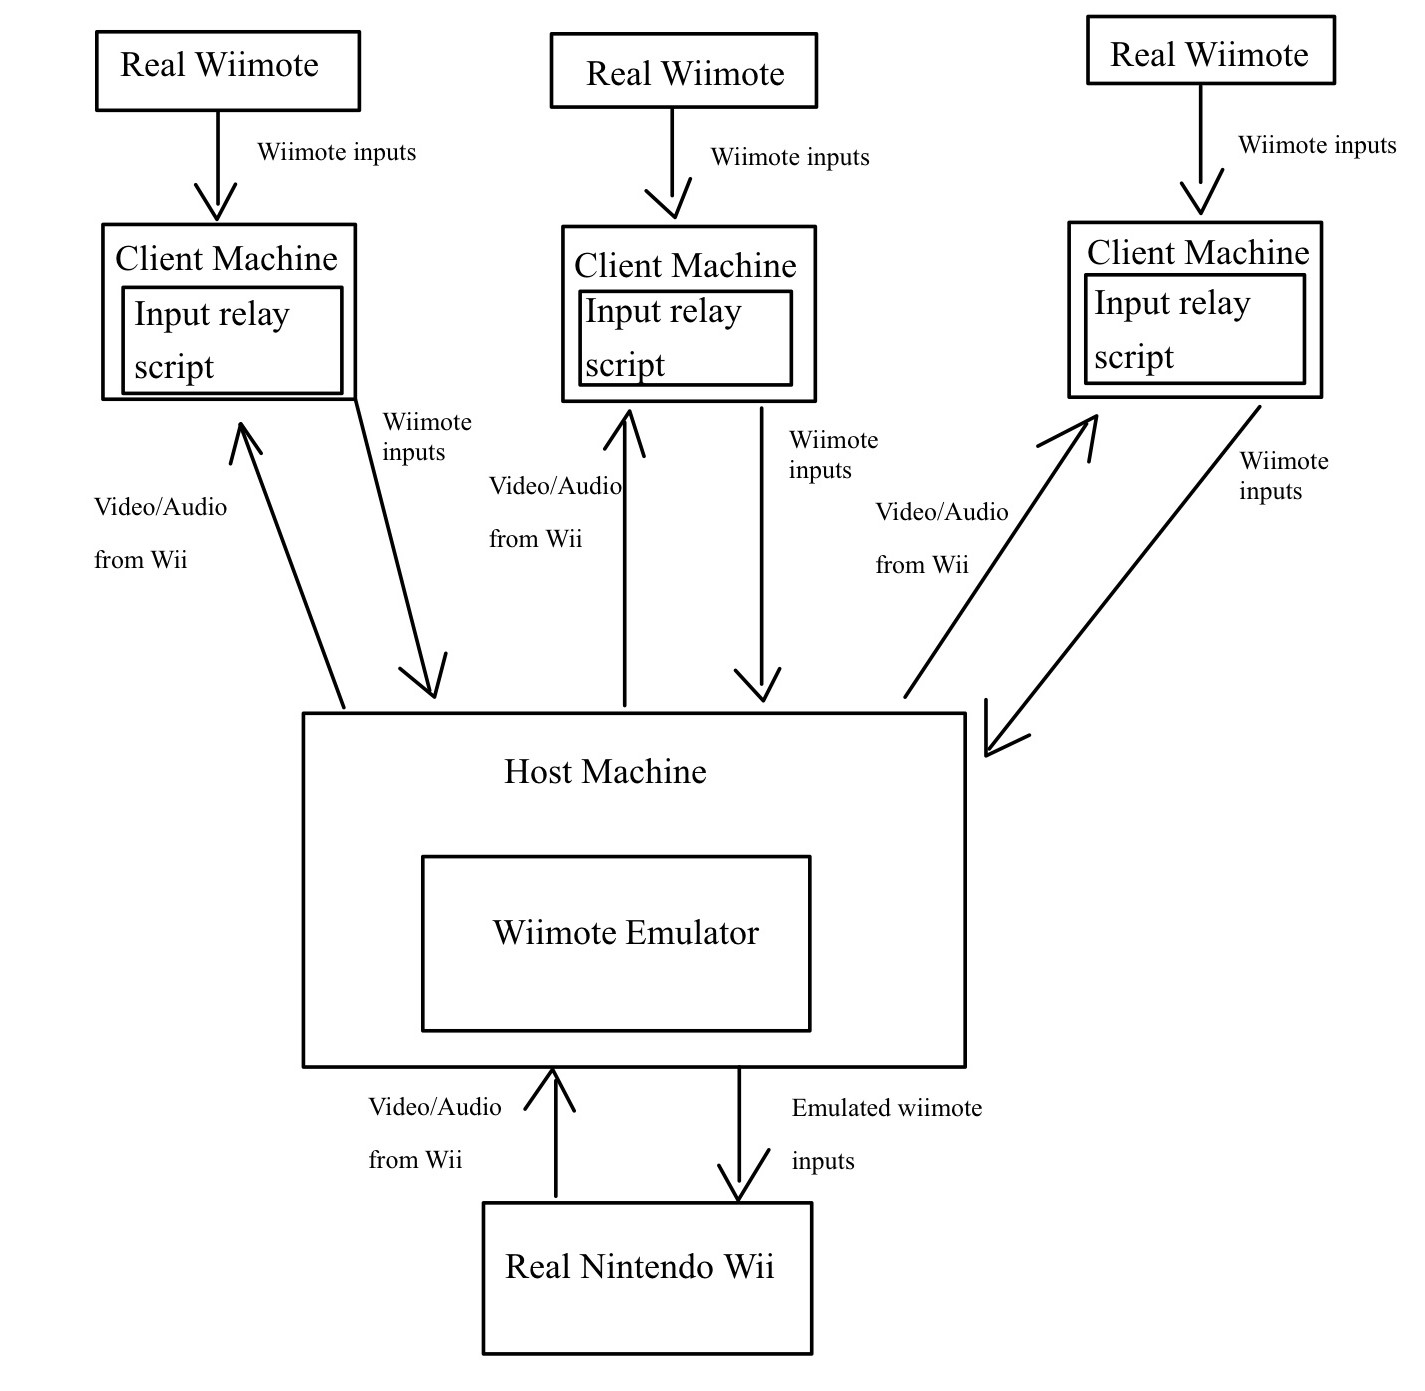
\includegraphics[width=0.8\textwidth]{diss_flow.jpg}
	\caption{System Architecture and Data Flow}
	\label{fig:architecture}
\end{figure}

At the core of the design is the input relay mechanism, which operates as follows:

\begin{enumerate}
	\item \textbf{Input Capture:}
	      The Wii Remote’s events are captured using the \texttt{xwiimote} library. Both analog (accelerometer, IR) and digital (button press) events are monitored continuously.

	\item \textbf{Event Processing:}
	      In the Python script, events are handled in a non-blocking manner using \texttt{select.poll()}. The script processes each event by normalising sensor data and mapping it into the expected range. For example, IR data is normalised to a [0,1] scale and then converted to a resolution that matches the Wii’s requirements, while accelerometer data is similarly scaled.

	\item \textbf{Packet Formation and Transmission:}
	      Processed events are packaged into binary data packets. The design utilises fixed-length packets with a dedicated header byte to distinguish between different types of events (e.g., \texttt{0x01} for IR and \texttt{0x02} for accelerometer data). These packets are transmitted over UDP to the emulator, which interprets them to simulate the corresponding inputs.

	\item \textbf{Emulation and Output:}
	      The emulator on the host Raspberry Pi receives the UDP packets and integrates the data into its internal state. The emulation layer uses transformation routines to convert the incoming data into the simulated state of the Wii Remote, including generating IR positions and accelerometer readings.
\end{enumerate}

\section{Unusual and Innovative Design Features}

Several aspects of the system’s design stand out due to their innovative nature:

\subsection{End-to-End Multiplayer Revival}

The system is designed to recreate the local multiplayer experience of the Nintendo Wii in an online setting. By combining audiovisual streaming with real-time input relay, the project aims to provide a seamless and authentic gaming experience that captures the essence of the original console. The project is easy to setup and use due to the automation scripts removing the need for advanced technical knowledge. This holistic approach to reviving the multiplayer capabilities of the Nintendo Wii is unique and distinguishes the project from other remote gaming solutions.


%% \subsection{Binary Protocol for Real-Time Communication}

%% Instead of relying on verbose text-based protocols, the system employs a custom binary protocol to transmit sensor and button events over UDP. This design decision minimises overhead and latency, which are critical for real-time input relay. By defining fixed packet structures and using network byte order for float values, the system achieves a high level of efficiency in both packing and unpacking data. Such low-level control over the communication protocol is uncommon in similar projects and represents a key innovation in the design.

\subsection{Modular and Extensible Input Processing}

The design of the input processing pipeline is highly modular. Different types of inputs (e.g., IR, accelerometer, button events) are handled in discrete sections of the code. This modularity allows for independent testing and future enhancements; for instance, additional sensor types or new control schemes can be incorporated with minimal changes to the overall architecture.

\subsection{Automated Environment Configuration}

Another unusual aspect of the design is the automated device setup. Recognising the complexity involved in configuring kernel modules, Bluetooth settings, and environment variables across multiple devices, an automation script was developed. This script ensures that all prerequisites for running the system are met without manual intervention, significantly reducing setup time and potential human errors.

%% \section{Design Trade-offs and Considerations}

%% Throughout the design process, several trade-offs were considered:

%% \begin{itemize}
%%     \item \textbf{Latency vs. Quality:}
%%           The dual requirements of maintaining low latency and high-quality audiovisual output necessitated careful balancing. The use of RTP with specific broadcast and play parameters emerged as the optimal solution, though some latency issues remain, particularly in the synchronisation between the input relay and the video stream.

%%     \item \textbf{Complexity vs. Modularity:}
%%           While modular design enhances maintainability and scalability, it also introduces complexity in terms of interfacing between different subsystems.

%%     \item \textbf{Performance vs. Flexibility:}
%%           The decision to implement performance-critical components in C ensures fast processing of sensor data but at the cost of reduced flexibility compared to a pure Python solution. The hybrid approach adopted here strikes a balance by enabling rapid development in Python for higher-level functions while reserving C for tasks where performance is paramount.
%% \end{itemize}
